\sujet{Geometry}

\noindent
Duration : 45mn - 10 points\\
{\bf Please, send your final codes to: \texttt{debayle@emse.fr}}\\


\section{Percolation}
\begin{figure}[htbp]
 \centering
 \subfloat[No percolation]{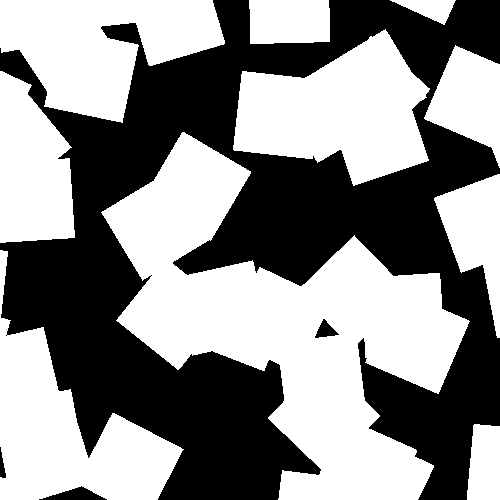
\includegraphics[width=4cm]{BW2.png}}\hspace*{0.5cm}
 \subfloat[North-south percolation]{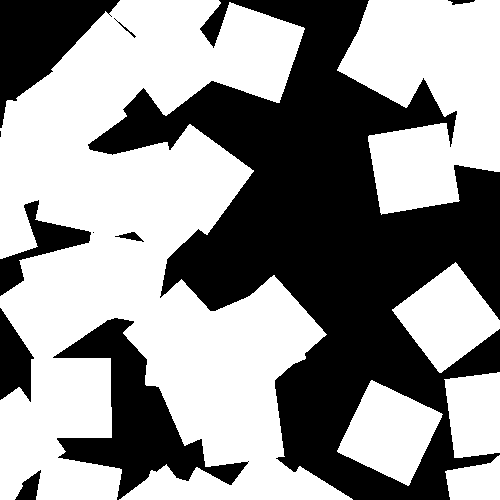
\includegraphics[width=4cm]{BW1.png}}\hspace*{0.5cm}
 \subfloat[West-east percolation]{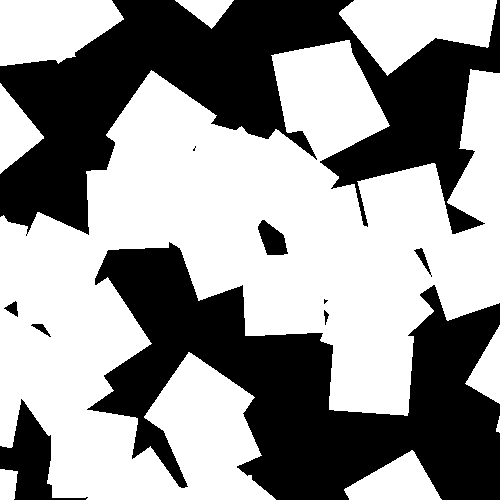
\includegraphics[width=4cm]{BW0.png}}
 \caption{Different realizations of a Boolean model of squared sets.}
 \label{fig:exam_2016:seeds}
\end{figure}

A spatial structure percolates when an aggregate of objects connects two opposite faces. In 2-D, one can look at the north-south and west-east faces. Some examples are given in Figure 1. 

\begin{qbox}
\begin{itemize}
\item Implement an automatic method to test if a 2-D spatial structure percolates (north-south and west-east directions).
\item Test your method on the three given images.
\item When it percolates, compute the ratio between the surface area of the connected component that percolates and the total surface area of the objects.
\end{itemize}
\end{qbox}

\begin{mcomment}
\begin{mremark}
You can use the function \minline{bwlabel} to identify the different connected components of a binary image. It could help you to check the percolation!
\end{mremark}
\end{mcomment}

